% Dokumentklasse, Papiergröße, Schriftgröße, keine Punkte am Ende der Kapitelnummerierung
\documentclass[a4paper,12pt, numbers=noendperiod]{scrreprt}
% Einstellung der Seitenrender, für Bindung geeignet
\usepackage[left= 2.5cm,right = 2cm, bottom = 4 cm]{geometry}
% Einstellung des zeilenabstandes, hier 1,5
\usepackage[onehalfspacing]{setspace}
% ============= Packages =============

\PassOptionsToPackage{hyphens}{url} % Für besseres URL handling bei Quellenangaben
% Dokumentinformationen
\usepackage[
	pdftitle={Titel der Arbeit},
	pdfsubject={},
	pdfauthor={Jane/John Doe},
	pdfkeywords={Vorlage, Abschlussarbeit},	
	ngerman
	% Links nicht einrahmen:
	%hidelinks
]{hyperref}


% Standard Packages
\usepackage[utf8]{inputenc}
\usepackage[ngerman]{babel}
\usepackage[T1]{fontenc}
\usepackage{graphicx, subfig}
\usepackage{fancyhdr}
\usepackage{lmodern}
\usepackage{color}
\usepackage{float}
\usepackage{capt-of}

% definiere Ordnernamen in dem Abbildungen abgelegt sind, dadurch ist im Folgenden nur noch ein führender Slash ('/') notwendig; Unterordner müssen weiterhin angegeben werden
\graphicspath{{img}}

%nummerierte Aufzählungen 
\usepackage{enumitem}

%Tabellen
\usepackage{longtable}
\usepackage{multirow}

%Zum drehen von Seiten
\usepackage{lscape}

%\usepackage{chngcntr}
%\usepackage[square]{natbib}

%Eine Hilfe zur Verwaltung von Abkürzungen
\usepackage[printonlyused]{acronym}

\usepackage{mathtools}

\usepackage{courier} %typewriter

% zusätzliche Schriftzeichen der American Mathematical Society
\usepackage{amsfonts}
\usepackage{amsmath}
\usepackage{esvect}

%nicht einrücken nach Absatz
\setlength{\parindent}{0pt}

%zwei bzw drei Zitate hintereinander
%\providecommand{\twocite}[4]{\citep[{\citealp[#1]{#2};}][#3]{#4}}
%\providecommand{\twocites}[3]{\citep[{\citealp{#1};}][#2]{#3}}
%\providecommand{\threecite}[6]{\citep[{\citealp[#1]{#2}; \citealp[#3]{#4};}][#5]{#6}}

%Überschriftenabstände einstellen
\renewcommand*\chapterheadstartvskip{\vspace*{-\topskip}}
\renewcommand*\chapterheadendvskip{%
	\vspace*{1\baselineskip plus .1\baselineskip minus .167\baselineskip}}

%Definition der Gliederungstiefe
\setcounter{secnumdepth}{5}
\setcounter{tocdepth}{5}

% ============= Python Umgebung =============
\usepackage{pythonhighlight}

% ============= Kopf- und Fußzeile =============
\pagestyle{fancy}

%
\lhead{}
\chead{}
\rhead{\slshape \leftmark}
%%
\lfoot{}
\cfoot{}
\rfoot[\thepage]{\thepage}
%%
\renewcommand{\headrulewidth}{0.4pt}
\renewcommand{\footrulewidth}{0.4pt}
\renewcommand*\chapterpagestyle{fancy}
% ============= Package Einstellungen & Sonstiges ============= 
%Besondere Trennungen
\hyphenation{De-zi-mal-tren-nung}

%römische Aufzählung
\newcommand{\RM}[1]{\MakeUppercase{\romannummeral #1}}
% ============= Dokumentbeginn =============

\begin{document}

%Seiten ohne Kopf- und Fußzeile sowie Seitenzahl
\pagestyle{empty}
\setlength{\parindent}{0pt}
\begin{center}
\begin{tabular}{p{\textwidth}}


\begin{center}

\includegraphics[width=10cm]{img/Administrativ/BUW_Logo.png}
\end{center}


\\

\begin{center}
\Large{\textsf{\textbf{
Fakultät für Architektur und Bauingenieurwesen\\
Lehrstuhl für Computational Civil Engineering\\
}}}
\end{center}

\\


\begin{center}
	\fontsize{40}{35}
	%Art der Abschlussarbeit
	\textsf{\textbf{\textit{Bachelor-/Masterthesis}}}
\end{center}
\\
\\
\\
\begin{tabular}{llp{12cm}}
	%Thema
	\textsf{\textbf{\Large{\underline{Thema:}}}} & & \textsf{\textbf{\Large{Vorlage zur Erstellung von Abschlussarbeiten}}}
\end{tabular}
\\
\\
\\
\begin{tabular}{lll}
\textsf{\textbf{Name:}} & & \textsf{Jane/John Doe}\\
\textsf{\textbf{Matrikelnummer:}} & & \textsf{1234567}\\
\textsf{\textbf{Anschrift:}} & & \textsf{Hauptstraße 123 in 12345 Musterstadt}\\
 & & \\
\textsf{\textbf{Hochschullehrer:}} & & \textsf{Prof. Dr. rer. nat. Lukas Arnold}\\
\textsf{\textbf{Betreuer:}} & & \textsf{Der zweite Betreuer}\\
 & & \\
\textsf{\textbf{Tag der Abgabe:}} & & \textsf{Datum}\\
\end{tabular}


\end{tabular}
\end{center}

% \part im Inhaltsverzeichnis nicht nummerieren
\makeatletter
\let\partbackup\l@part
\renewcommand*\l@part[2]{\partbackup{#1}{}}

%Seitennummerierung neu beginnen
\pagenumbering{Roman}

%\pagestyle{plain}
\pagestyle{fancy}

\include{020_Erklärung}

\addsec{Kurzfassung}
\rhead{\slshape Kurzfassung}
\label{Kurzfassung}

Hier soll eine Kurzfassung der Arbeit stehen. Das heißt was wurde gemacht und zu welchem Ergebnis führt dies. Welche neuen wissenschaftlichen Erkenntnisse konnten gewonnen werden? Diese sollte sich auf 200 Worte beschränken.

\newpage
\addsec{Abstract}
\rhead{\slshape Abstract}
\label{Abstract}

Here should be a abstract of the thesis in English. That is, what was done and to what result this leads. What new scientific knowledge has been gained? This should be limited to 200 words.


\newpage

% pagestyle für gesamtes Dokument aktivieren
\pagestyle{fancy}

%Inhaltsverzeichnis
\addcontentsline{toc}{section}{Inhaltsverzeichnis}
\rhead{\slshape Inhaltsverzeichnis}
\tableofcontents


%Abkürzungsverzeichnis
\chapter*{Nomenklatur}
\label{AKV}
\addcontentsline{toc}{section}{Nomenklatur} 
\rhead{\slshape Nomenklatur}
\section*{Formelzeichen}
\addcontentsline{toc}{subsection}{Formelzeichen}

\begin{longtable}{p{1.5cm}p{11cm}l}
% Liste der verwendeten Formelzeichen in Alphabetischer Reihenfolge	
	\textbf{Symbol} 	& \textbf{Bedeutung} 			& \textbf{Einheit} \endhead \\ %Headline
	$\vec{\mathsf{f}}$	& Volumenkraftdichte			& N / $\mathrm{m^3}$ \\
	$\lambda$			& erste Lamé-Konstante			& Pa \\
	$\mu$				& Dynamische Viskosität			& Pa $\cdot$ s \\
	p					& (statischer) Druck			& Pa \\
	$\rho$ 				& Dichte 						& kg /$\mathrm{m^3}$ \\
	$\vec{\mathsf{v}}$	& Geschwindigkeit				& m / s \\

	
		
\end{longtable}

%%%%%%%%%%%%%%%%%%%%%%%%%%%%%%%%%%%%%%%%%%%%%%%%%%%%%%%%%%%%%%%%%%%

\section*{Abkürzungen}
\addcontentsline{toc}{subsection}{Abkürzungen}

\begin{acronym}[FDS]
	\acro{FDS}{Fire Dynamics Simulator}
	
\end{acronym}

\rhead{\slshape \leftmark}

%Verzeichnis aller Bilder
\listoffigures
\addcontentsline{toc}{section}{Abbildungsverzeichnis}

%Verzeichnis aller Tabellen
\listoftables
\addcontentsline{toc}{section}{Tabellenverzeichnis}

\newpage
%%%%%%%%%%%%%%%%%%%%%%%%%%%%%%%%%%%%%%%%%%%%%%%%%%%%%%%%%%%%%

%Seitennummerierung neu beginnen
\pagenumbering{arabic}

\pagestyle{fancy}

\chapter{Einleitung}
\label{cpt:Einleitung}

\section{Problemstellung}
\label{sec:Problemstellung}

Was soll thematisiert werden?\\
Die Empfohlene Anzahl an Seiten für eine Bachelorarbeit liegt bei etwa 40 und etwa 60 für eine Masterarbeit. Ausführliche Tabellen, Quellcode oder Rohdaten sollten Teil des Anhangs sein um das Lesen des Hauptdokumentes übersichtlicher zu machen. 

\section{Zielsetzung}
\label{sec:Zielsetzung}

In der Regel steht hier so etwas wie die Motivation.

\section{Abgrenzung}
\label{sec:Abgrenzung}

Was wird betrachtet und was nicht, warum wird die Grenze genau an der Stelle gezogen?\\
Dabei sollte die eigene Arbeit auch gegen andere Arbeiten abgegrenzt werden. Hierfür ist eine Literaturrecherche unerlässlich. Für die Literaturrecherche können beispielsweise folgende Suchmaschinen einen Anfangspunkt bilden, diese sind besonders geeignet um Paper und andere wissenschaftliche Veröffentlichungen zu finden, wie z.B. \cite{Hehnen.2020}:
\begin{itemize}[itemsep=-6pt]
	\item \url{https://scholar.google.de/}
	\item \url{https://www.sciencedirect.com/}
	\item \url{https://www.ulb.uni-muenster.de/lotse/}
	\item \url{https://www.springer.com/gp}
\end{itemize}

Weitere Hinweise zu Inhalten von Kapiteln, möglichem Aufbau der Arbeit sowie Hinweise zum wissenschaftlichen Schreiben können der Präsentation zur Vorlesung \glqq Einführung in das wissenschaftliche Schreiben\grqq entnommen werden. Diese steht öffentlich zum Download unter folgender Adresse zur Verfügung.
\url{https://www.asim.uni-wuppertal.de/de/lehre/wissenschaftliches-schreiben.html}

\section{Herangehensweise}
\label{sec:Herangehensweise}

Welche Hilfsmittel werden verwendet z.B. \ac{FDS}, FDSReader, PROPTI.

\chapter{Methoden}
\label{cpt:Methoden}

Vorstellung des Standes der Technik und Wissenschaft anhand bereits existierender Normen und wissenschaftlicher Arbeiten. Sowie eine knappe Beschreibung der Methoden, die für diese Arbeit relevant sind und über den durchschnittlichen Kenntnisstand des Lesers hinaus gehen. \\

Bei der Verwendung dieser vierteiligen Gliederung bestehend aus:
\begin{enumerate}[itemsep=-6pt]
	\item Einleitung
	\item Methoden
	\item Ergebnisse
	\item Diskussion
\end{enumerate}
gehören in den Methoden Teil auch die eigenen Arbeiten mit den folgenden Inhalten.
\begin{itemize}[itemsep=-6pt]
	\item Dokumentation der eigenen Arbeiten
	\item Auflistung der verwendeten Methoden und deren Parameter
	\item Verifikation, Validierung und Plausibilität der Methoden und Parameter
	\item Struktur und Vorgehensweise
	\item Exemplarische oder charakteristische Rohdaten präsentieren
\end{itemize}

Dabei werden z.B. die verwendeten Formeln wie hier \autoref{equ:Nav} dargestellt.

\begin{equation}
	\label{equ:Nav}
	\mathrm{\partial_t} \rho \vec{\mathsf{v}} + \nabla \cdot (\rho \vec{\mathsf{v}} \vec{\mathsf{v}}) = -\nabla \mathsf{p} + \mu \nabla^2 \vec{\mathsf{v}} + \vec{\mathsf{f}} 
\end{equation}

Es können auch Aufzählungen verschiedener Arten verwendet werden. Hierbei sollte darauf geachtet werden, dass die Abstände zwischen Punkten der gleichen Gliederungsstufe den gleichen Zeilenabstand haben wie der übrige Text. 

\begin{itemize}[itemsep=-6pt]
	\item erste Ebene
	\begin{itemize}[itemsep=-6pt]
		\item zweite Ebene
		\item auch zweite Ebene
		\begin{itemize}[itemsep=-6pt]
			\item dritte Ebene
			\begin{itemize}[itemsep=-6pt]
				\item vierte Ebene
			\end{itemize}
		\end{itemize}
	\end{itemize}
\end{itemize}

\begin{itemize}[itemsep=-6pt]
	\item[-] ein selbst gewähltes Aufzählungszeichen
	\item[\#] ein anderes selbst gewähltes Aufzählungszeichen
\end{itemize}



\chapter{Ergebnisse}
\label{cpt:Ergebnisse}

Hier werden die eigenen Ergebnisse dargestellt. Die Eigenleistung sollte im Fokus stehen und somit auch den größten Teil der Arbeit ausmachen. 

Die Ergebnispräsentation kann durch graphische Darstellungen häufig gut unterstützt werden (vgl. \autoref{fig:Vgl_Exp_1_2}).
Besonders schön ist es dabei, wenn in der Graphik die gleiche Schriftart Verwendung findet wie sie im Text verwendet wird. Ebenfalls für einen besonders sauberen optischen Eindruck sorgen Vektorgrafiken. Gerade in den gedruckten Exemplaren fügen sich diese besser in das hochauflösende Schriftbild der Texte ein. Bei der Erstellung von Graphiken mit Python ist dies durch die Verwendung von \LaTeX -rendering möglich. Der Quelltext für \autoref{fig:Vgl_Exp_1_2} befindet sich in \autoref{Quelltext_A}. 

\begin{figure}[H]
	\centering
	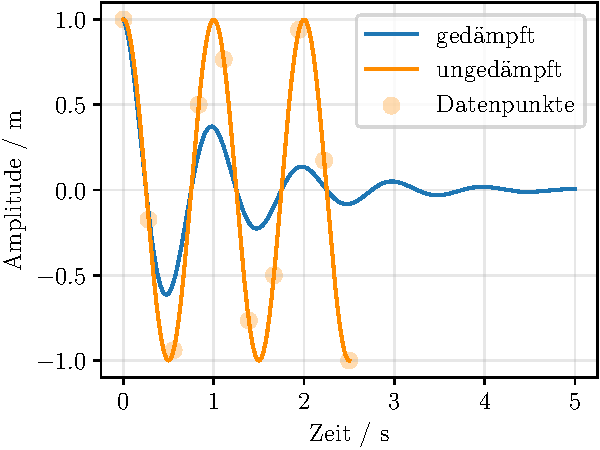
\includegraphics[scale=1]{/Schwingungen.pdf}
	\caption[Darstellung verschiedener Kosinunsschwingungen]{Darstellung einer gedämpften und einer ungedämpften Kosinusschwingung}
	\label{fig:Vgl_Exp_1_2}
\end{figure}

Es kann sinnvoll oder sogar notwendig sein, dass Daten geglättet oder zum Beispiel aufgrund physikalischer Zusammenhänge bestimmte Funktionen angenommen werden. Dabei ist es wichtig dem Betrachter der Graphik nicht zu suggerieren, dass die bearbeitete Darstellung den Messwerten entspricht. Um dies zu vermeiden sollten die tatsächlichen Datenpunkte mit dargestellt werden, wie in \autoref{fig:Vgl_Exp_1_2} am Beispiel der ungedämpften Schwingung dargestellt. Ist die Punktdichte sehr hoch und die Daten wurden nicht bearbeitet, ist dies nicht erforderlich, da es keinen informativen Mehrwert bietet.\\ 

Lässt sich die Unsicherheit der Daten angeben kann diese Beispielsweise durch graue Einfärbungen in die Graphik integriert werden und bietet so einen schnellen Überblick (vgl. \autoref{fig:Unsicherheit}), der Quelltext befindet sich in \autoref{Quelltext_B}. 

\begin{figure}[H]
	\centering
	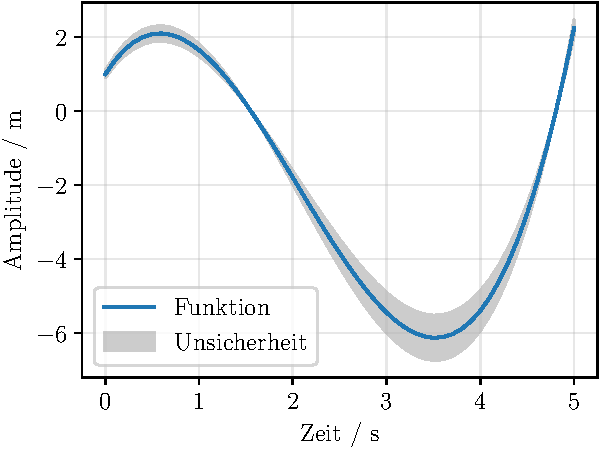
\includegraphics[scale=1]{/Fkt_mit_Unsicherheit.pdf}
	\caption{Darstellung einer Funktion mit Angabe des Unsicherheitsbereiches}
	\label{fig:Unsicherheit}
\end{figure}

Neben den bereits vorgestellten Graphen können auch andere Darstellungsformen Verwendung finden. In \autoref{fig:Boxplot} sind Beispielhaft Boxplots dargestellt. Die Darstellungsform sollte sorgsam gewählt werden um den Betrachter beim erfassen der relevanten Informationen so gut wie möglich zu unterstützen.

\begin{figure}[H]
	\centering
	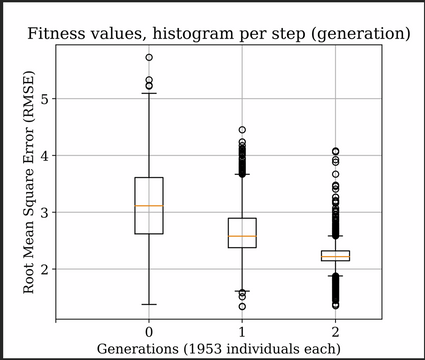
\includegraphics[scale=.5]{/Boxplot.png}
	\caption{Darstellung mehrerer Boxplots}
	\label{fig:Boxplot}
\end{figure}

Auch Tabellen können einen guten Überblick über die Arbeit ermöglichen (vgl. \autoref{tab:example}). Diese können auch mit verschiedenen \href{https://www.tablesgenerator.com/}{Online Tools} vorformatiert werden , dies ist insbesondere dann sinnvoll, wenn die Tabellenköpfe etwas verschachtelter sind.

\begin{table}[H]
	\caption{Das ist ein Beispiel für eine Tabelle}
	\label{tab:example}
	\begin{tabular}{|l|l|l|l|l|}
		\hline
		\multicolumn{1}{|c|}{\multirow{2}{*}{\textbf{NR.}}} & \multicolumn{2}{c|}{\textbf{Kategorie 1}}               & \multicolumn{2}{c|}{\textbf{Kategorie 2}}               \\ \cline{2-5} 
		\multicolumn{1}{|c|}{}                              & \textit{Unterkategorie 11} & \textit{Unterkategorie 12} & \textit{Unterkategorie 21} & \textit{Unterkategorie 22} \\ \hline
		1	&                            &                            &                            &                            \\ \hline
		2	&                            &                            &                            &                            \\ \hline
	\end{tabular}
\end{table}

Den Abschluss des Kapitels der Ergebnisse sollte die Einordnung der Ergebnisse in den wissenschaftlichen Gesamtkontext bilden. 


\chapter{Diskussion}
\label{cpt:Diskussion}

Die Diskussion stellt eine kritische Betrachtung der eigenen Arbeit dar. Es sollen Probleme aufgezeigt werden und Ansätze zur Verbesserung gegeben werden. Darüber hinaus können Ansätze zur Erweiterung der Arbeit vorgestellt werden, die Potential für weitere Arbeiten in die gleiche Richtung aufzeigen. 

\chapter{Zusammenfassung}
\label{cpt:Zusammenfassung}

Abschließend folgt eine Zusammenenfassung, die den Umfang des Abstracts deutlich übersteigen sollte. Hier sind 2 - 3 Seiten anzustreben.

%Literaturverzeichnis
\newpage
\addcontentsline{toc}{chapter}{Literatur}
\bibliography{Literatur}
\bibliographystyle{unsrtdin}

%%%%%%%%%%%%%%%%%%%%%%%%%%%%%%%%%%%%%%%%%%%%%%%%%%%%%%%%%%%%%%%%%
% \part im Inhaltsverzeichnis nicht nummerieren
\newpage
\makeatletter
\let\partbackup\l@part
\renewcommand*\l@part[2]{\partbackup{#1}{}}

%Seitennummerierung neu beginnen
\pagenumbering{roman}

\clearpage
\appendix

\chapter{Quelltext}
\label{Quelltext_A}

\inputpython{scripts/schwingungen.py}{1}{39}

\chapter{Quelltext}
\label{Quelltext_A}

\inputpython{scripts/fkt_mit_unsicherheit.py}{1}{39}



\end{document}
